
Una vegada havia implementat la distància de Férchet per poder avaluar el rendiment dels models, vaig arribar a una clara conclusió:

Els models que tenen implementada la funció no lineal són més eficients. 

Afirmo això perquè els models sense la funció no arriben a estabilitzar-se, és a dir, no arriben al punt d'equilibri. En canvi, els models que tenen la funció si ho fan. Arribar al punt d'equilibri garanteix que les imatges generades siguin com les reals. Per molt més que el model segueixi optimitzant-se, sempre donarà les millors imatges generades. 

Els models que no presenten la funció no assoleixen aquest punt a causa que la semblança de les imatges oscil·la, és a dir, el model pot arribar a generar imatges correctament, però no ho fa indefinidament, al cap d'unes interaccions la semblança de les imatges generades amb les reals ja no és significativa. Simplement, la qualitat de les imatges generades va oscil·lant entre bona i dolenta. Tot i que hi ha excepcions, a vegades els models sense la funció no experimenten aquesta oscil·lació. Tanmateix cal remarcar que les vegades que passa són notablement més altes que les que no passa. Com es pot veure amb les dades de la taula \ref{tab:oscilations}.

Aquest problema no és causat pel discriminador, això és perquè la variable independent de l'experiment és el circuit quàntic del generador, per tant, és el factor que té més possibilitat de ser el causant d'aquest comportament. No sé molt bé la causa exacta, però està clar que el mesurament parcial té un impacte.

\begin{table}[H]
	\resizebox{\textwidth}{!}{%
		\begin{tabular}{c|c|c}
			\hline
			& Presenta oscil·lació & No Presenta oscil·lació \\
			\hline
			Amb Funció No Lineal & 0 & 6 \\
			\hline
			Sense Funció No Lineal& 5 & 1 \\
			\hline
		\end{tabular}
	}
	\caption{Les dades provenen d'un total de 6 models, 3 d'ells amb un total de $700$ iteracions i els altres 3 amb un total de $550$. El nombre d'interaccions no hauria d'afectar de cada manera les dades. Degut si hi ha una oscil·lació, es pot veure clarament a partir de les $400$ iteracions. Amb les dades es pot veure que és més probable que un model sense la funció lineal presenti una oscil·lació. Cal notar que cap model amb la funció ha tingut una oscil·lació. Les gràfiques que corresponen a cada model es poden veure en les figures \ref{fig:700_SD_score} i \ref{fig:550_SD_score}.}
	\label{tab:oscilations}
\end{table}

\begin{figure}[H]
	\begin{subfigure}[b]{.32\linewidth}
		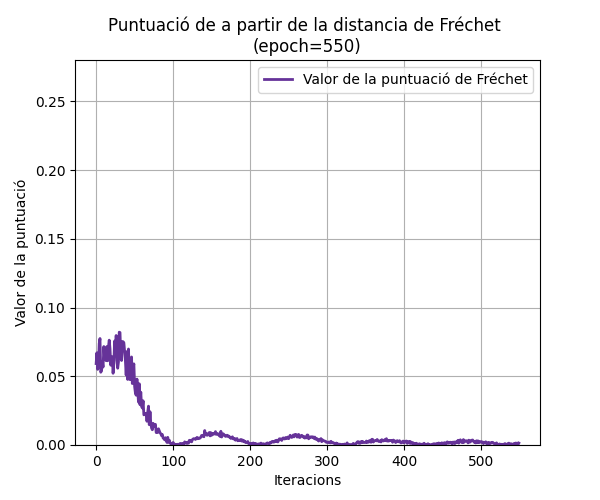
\includegraphics[width=\linewidth]{figures/data/FD_score_1.png}
		\caption{}
	\end{subfigure}
	\begin{subfigure}[b]{.32\linewidth}
		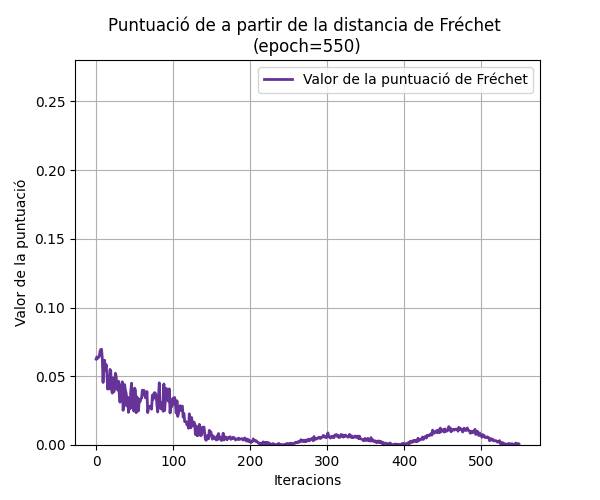
\includegraphics[width=\linewidth]{figures/data/FD_score_2.png}
		\caption{}
	\end{subfigure}
	\begin{subfigure}[b]{.32\linewidth}
		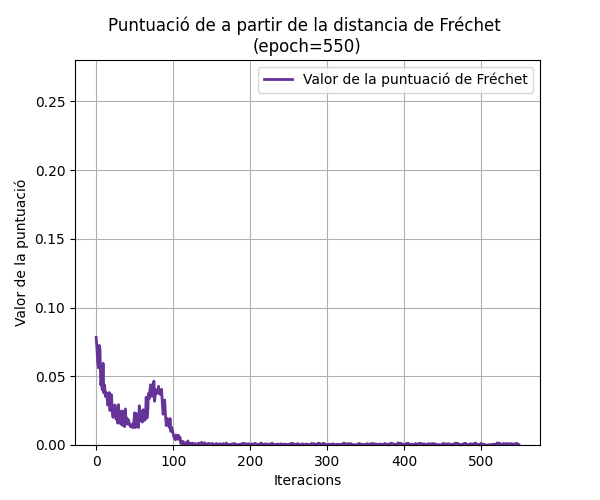
\includegraphics[width=\linewidth]{figures/data/FD_score_3.png}
		\caption{}
	\end{subfigure}
	
	\begin{subfigure}[b]{.32\linewidth}
		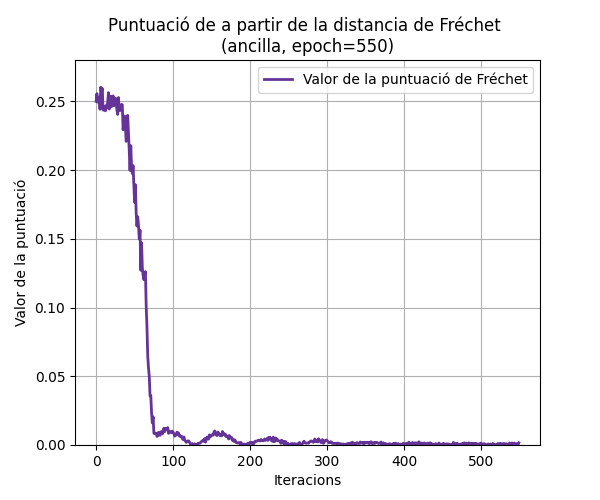
\includegraphics[width=\linewidth]{figures/data/FD_score_A1.png}
		\caption{}
	\end{subfigure}
	\begin{subfigure}[b]{.32\linewidth}
		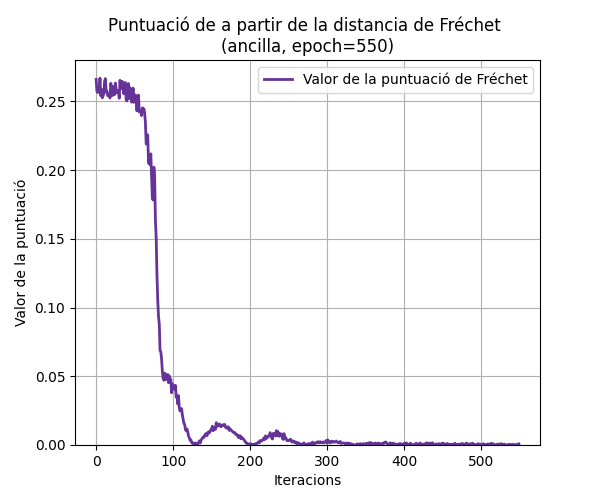
\includegraphics[width=\linewidth]{figures/data/FD_score_A2.png}
		\caption{}
	\end{subfigure}
	\begin{subfigure}[b]{.32\linewidth}
		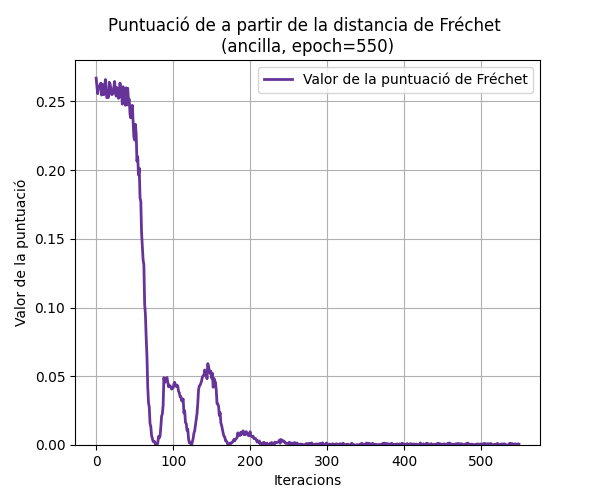
\includegraphics[width=\linewidth]{figures/data/FD_score_A3.png}
		\caption{}
	\end{subfigure}
	\caption{Totes les gràfiques corresponen a models que s'ha executat al llarg de $550$ iteracions. Les figures \textbf{A}, \textbf{B} i \textbf{C}, corresponen a models sense la funció lineal. L'únic d'ells que no presenta una oscil·lació és el \textbf{C}. Les gràfiques sense la funció es poden comparar a les d'abaix, les quals representen models amb la funció implementada. Els models han estat creats per parelles, les quals estan organitzades verticalment. És a dir, les gràfiques \textbf{A} i \textbf{D} representen models que tenen els mateixos paràmetres inicials. El mateix passa amb \textbf{B} i \textbf{E} i amb \textbf{C} i \textbf{F}.}
\label{fig:550_SD_score}
\end{figure}

\begin{figure}[H]
	\begin{subfigure}[b]{.32\linewidth}
		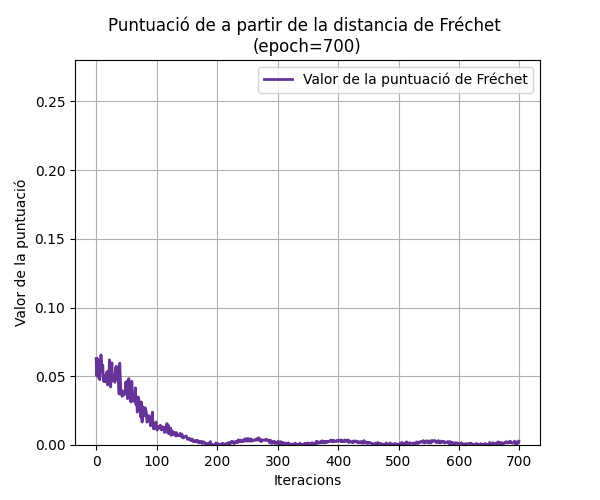
\includegraphics[width=\linewidth]{figures/data/FD_score_4.png}
		\caption{}
	\end{subfigure}
	\begin{subfigure}[b]{.32\linewidth}
		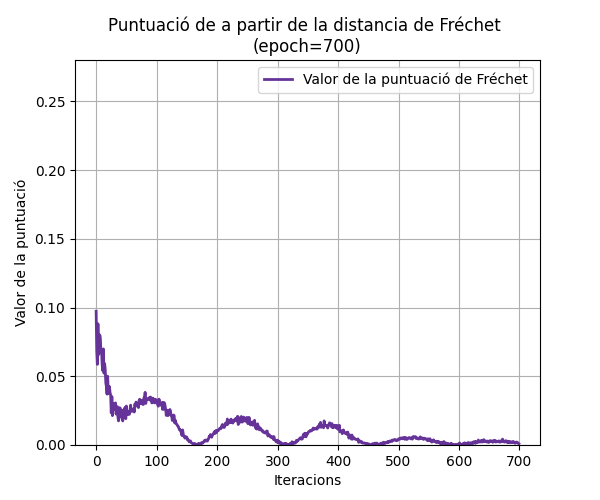
\includegraphics[width=\linewidth]{figures/data/FD_score_5.png}
		\caption{}
	\end{subfigure}
	\begin{subfigure}[b]{.32\linewidth}
		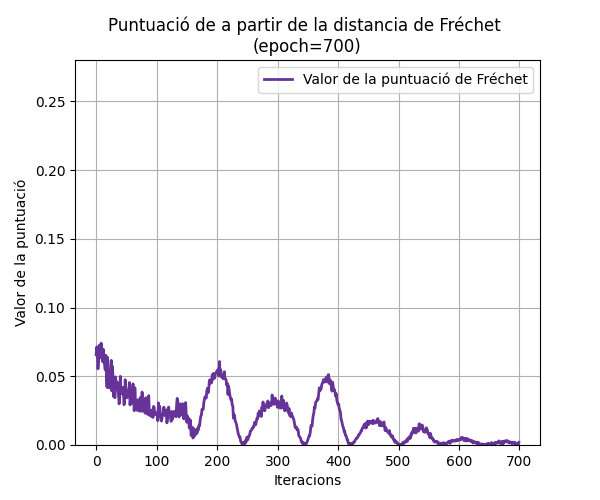
\includegraphics[width=\linewidth]{figures/data/FD_score_6.png}
		\caption{}
	\end{subfigure}
	
	\begin{subfigure}[b]{.32\linewidth}
		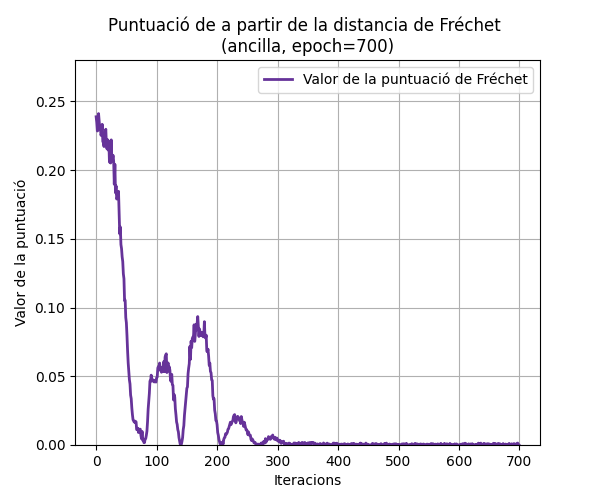
\includegraphics[width=\linewidth]{figures/data/FD_score_A4.png}
		\caption{}
	\end{subfigure}
	\begin{subfigure}[b]{.32\linewidth}
		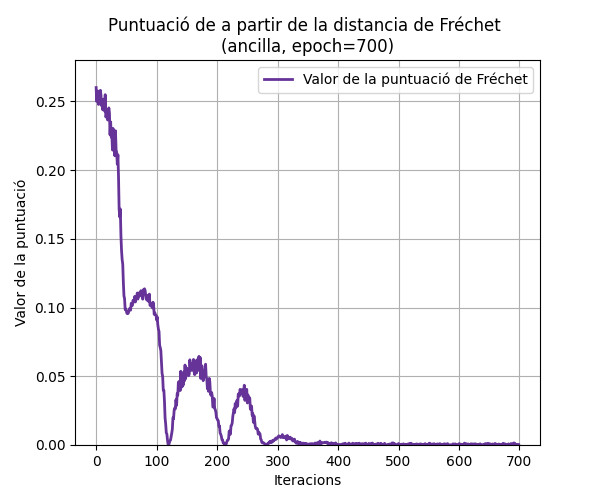
\includegraphics[width=\linewidth]{figures/data/FD_score_A5.png}
		\caption{}
	\end{subfigure}
	\begin{subfigure}[b]{.32\linewidth}
		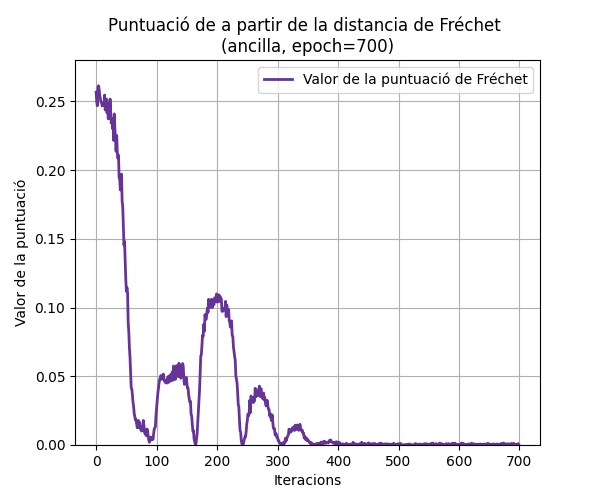
\includegraphics[width=\linewidth]{figures/data/FD_score_A6.png}
		\caption{}
	\end{subfigure}
	\caption{Aquestes gràfiques corresponen a models que s'han executat al llarg de $700$ iteracions. Estan organitzades igual que les gràfiques de la figura \ref{fig:550_SD_score}. En aquests casos, com es pot observar tots els models sense la funció no lineal presenten les oscil·lacions. No obstant això, en la gràfica \textbf{A}, aquesta es molt feble. Per veure com afecten les oscil·lacions es pot veure la figura \ref{fig:700_images}, on estan representades les últimes imatges que han generat els models que corresponen les gràfiques d'aquesta figura.}
	\label{fig:700_SD_score}
\end{figure}

En les gràfiques \ref{fig:550_SD_score} i \ref{fig:700_SD_score} es pot veure perfectament l'oscil·lació en la Distància de Fréchet. Es pot interpretar aquesta mètrica com la semblança entre les imatges generades i les reals. Si aquesta mètrica convergeix a zero, es pot dir que el model ha arribat al seu punt d'equilibri. Es pot veure com tots els models que tenen el mesurament parcial assoleixen aquest punt. D'aquesta manera demostrant l'eficàcia de la funció no lineal.

\begin{figure}[H]
	\begin{subfigure}[b]{.32\linewidth}
		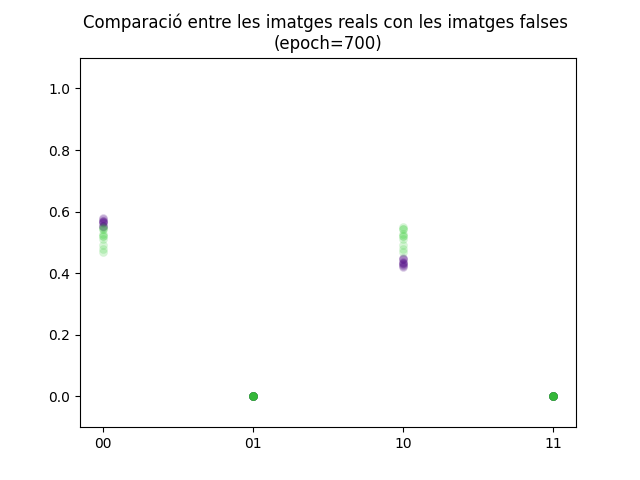
\includegraphics[width=\linewidth]{figures/data/scatter_plot_4.png}
		\caption{}
	\end{subfigure}
	\begin{subfigure}[b]{.32\linewidth}
		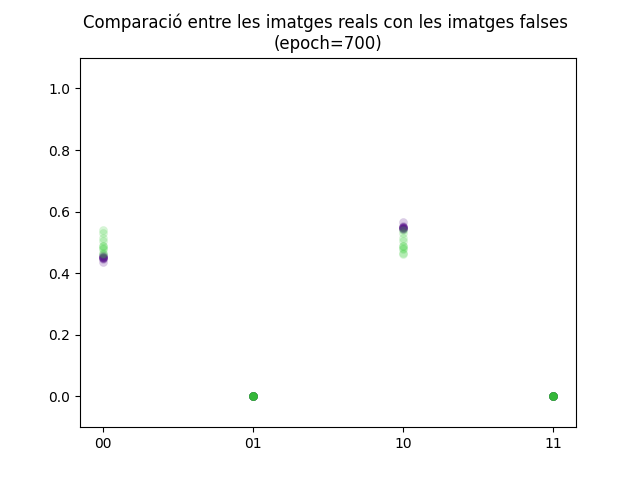
\includegraphics[width=\linewidth]{figures/data/scatter_plot_5.png}
		\caption{}
	\end{subfigure}
	\begin{subfigure}[b]{.32\linewidth}
		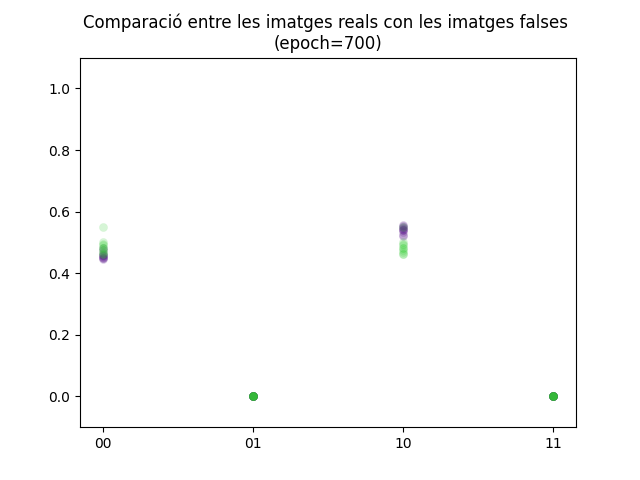
\includegraphics[width=\linewidth]{figures/data/scatter_plot_6.png}
		\caption{}
	\end{subfigure}
	
	\begin{subfigure}[b]{.32\linewidth}
		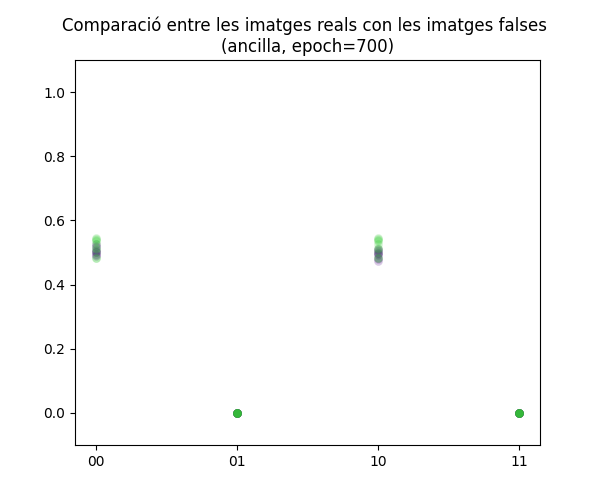
\includegraphics[width=\linewidth]{figures/data/scatter_plot_A4.png}
		\caption{}
	\end{subfigure}
	\begin{subfigure}[b]{.32\linewidth}
		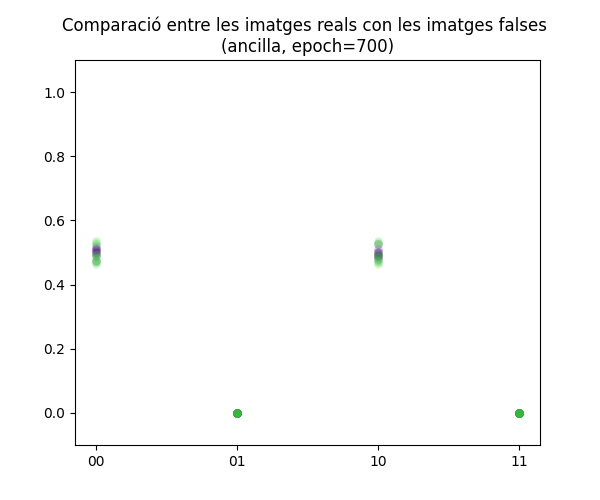
\includegraphics[width=\linewidth]{figures/data/scatter_plot_A5.png}
		\caption{}
	\end{subfigure}
	\begin{subfigure}[b]{.32\linewidth}
		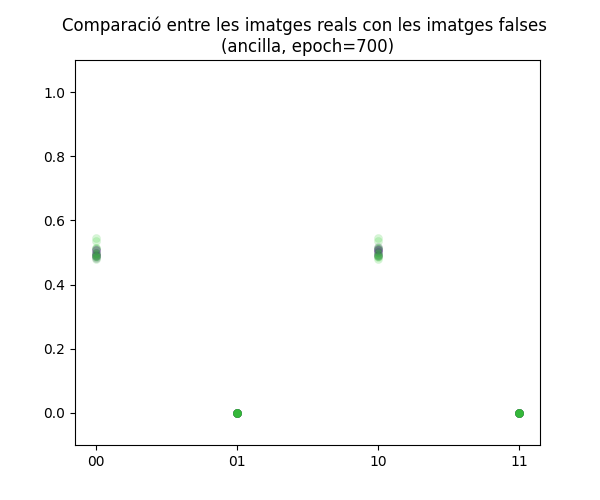
\includegraphics[width=\linewidth]{figures/data/scatter_plot_A6.png}
		\caption{}
	\end{subfigure}
	\caption{Aquestes gràfiques corresponen als mateixos models que els de la figura \ref{fig:700_SD_score}. Les posicions de les gràfiques són les mateixes, per tant, si estan en la mateixa posició que les de l'altra figura, corresponen al mateix model. Les imatges generades pels models sense la funció no lineal (\textbf{A}, \textbf{C}, \textbf{B}) no s'assemblen a les reals. Es pot veure com els punts de les imatges generades (color violeta) no estan als mateixos valors. Mentre que en les gràfiques \textbf{D}, \textbf{E} i \textbf{F}, sí que ho estan. Els punts violetes sembla que representen la mitjana dels punts verds. També es pot observar que les imatges generades tendeixen a ser més variades que les reals.}
	\label{fig:700_images}
\end{figure}

La diferència entre les imatges es pot veure la figura \ref{fig:700_images}, en la qual es mostren les 10 últimes imatges generades pels models optimitzats al llarg de 700 iteracions.

A partir de la Distància de Fréchet es pot apreciar l'efecte que té el mesurament parcial en la generació de les imatges, fent que aquest procés sigui més eficient i evitant una oscil·lació entre la generació d'imatges de bona i dolenta qualitat. Per tant, es pot afirmar que el mesurament té un efecte positiu en el model, corroborant la tesi exposada en Huang et. al. (2021) \cite{QGAN_exp}. 

No obstant això, es podria desenvolupar aquest experiment en major profunditat. No he tingut en compte el temps en el qual es tarden a generar les imatges. Els models amb el mesurament parcial implementat són més eficients, però en tenir més qubits és més costos simular-los i, per tant, tarden més temps per cada interacció. He fallat en mirar exactament quina és la diferència en termes de temps, tanmateix, ja que els models sense la funció no lineal no arriben a assolir el punt d'equilibri la gran majoria de les vegades, des d'un punt pràctic és recomanable utilitzar els models que si tenen la funció. 

A més a més es podria investigar la causa de l'oscil·lació en major profunditat. Deixant de banda la investigació teòrica de per què passa, es podria variar el nombre de qubits en els circuits, tant els ancilla, com el total de qubits del circuit, per veure quin és l'efecte que té tenir més qubits en el sistema ancilla. Potser investigaré pel meu compte aquesta qüestió. 

\section*{El camí que he recorregut}
Vull dedicar un petit espai per poder parlar sobre que significa aquest treball per a mi, de tot l'esforç que he posat en aquest, i finalment comentar tot el que he après.

Fa més de dos anys que vaig començar a aprendre conceptes de computació quàntica, ha sigut un camí molt llarg, però que m'ha encant recórrer. Pensar en tot el que he après em dona una gran alegria. Els camps dels quals he parlat realment m'encanten (computació quàntica i intel·ligència artificial). Aprendre tot això m'ajudaria molt en cas que estudiï una carrera en física, que és el meu objectiu. A més a més, alhora de realitzar el petit experiment m'he donat compte de la paciència necessària per poder desenvolupar experiments mitjançant el mètode científic. S'ha d'anar amb molta cura per assegurar-se de que la variable dependent no fossi afectada per les variables de control. Revisant una vegada i una altra fins a estar segur del resultats obtinguts. 

Deixant d'una banda els evidents beneficis d'avançar temari d'una carrera que vols fer en un futur, fent aquest treball he après altres coses extremadament útils.

Primer de tot, aquest treball està redactat en \LaTeX\footnote{\href{https://www.latex-project.org/}{La web oficial de \LaTeX}}, una espècie de llenguatge de programació per escriure equacions matemàtiques i documents de text. És àmpliament utilitzat per escriure articles científics en el món acadèmic, però més important, és utilitzat en l'ambient educatiu de les ciències exactes per poder entregar deures, reports del laboratori, i fer apunts. Tots els meus amics que estudien física o matemàtiques el fan servir.

A continuació està el fet de crear un gran projecte científic en \textit{Python}, he après a programar fins al punt que crec que soc bastant bo, és allò que se'm dona millor diria. Programar en \textit{Python} també és una habilitat que em serà útil a la universitat, perquè és el llenguatge de programació que es fa servir en la carrera de Física a la UB per realitzar experiments computacionals. Però, també vull mencionar que al llarg del procés de la creació del model van sorgir moltíssims problemes, en aquest document només he esmenat una part petita dels problemes que em vaig trobar al llarg del camí. Vaig estar més de mig any programant aquest model fins que estava tot perfecte per fer l'experiment. Definitivament, ha sigut la part més dura de tot el treball.

Per últim lloc, he après a llegir articles científics sobre computació quàntica i intel·ligència artificial. Estic familiaritzat amb la notació que s'empra en aquest camp i també el llenguatge específic que s'utilitza en els articles, amb això em refereixo a les expressions en anglès. No obstant això, hi ha coses que no puc arribar a comprendre és clar. No tinc els mateixos coneixements d'un estudiant de postgrau de física, matemàtiques o ciències de la computació. I no tinc la intenció d'afirmar que puc valorar els articles d'alguna manera, tan sols puc comprendre'ls fins a un nivell que ha estat suficient per a la realització d'aquest treball.

Aquest treball de recerca s'ha acabat, quan en realitat, és el començament del meu camí en la física, la computació quàntica, les ciències de la computació i la programació científica. La vida universitària em donarà més eines i aprenentatges per poder, de mica en mica, aprofundir i revisar tot el que he après al llarg d'aquest camí. 


%Deixant de banda els aspectes més positius de l'elaboració del treball, sí que considero que he fet alguns errors. 

%Primer de tot, no he demanat ajuda un professional de l'àmbit, quan perfectament podria haver-ho fet. He de reconèixer que no m'hauria costat tant de temps desenvolupar el model. També hauria tingut suport i guia a l'hora de consultar articles científics. Per aquesta raó penso, en un futur, mirar a tot el que he après en aquest viatge com coneixements que s'han de qüestionar, d'aquesta manera progressaré. 

%En segon lloc, si pogués tornar enrere en el temps, hauria creat el repositori de \textit{Github} des d'un principi. D'aquesta manera podria haver-hi un bon diari per recopilar el progrés i l'evolució del codi. Penso que he parlat molt poc del procés de creació del model, i que no li vaig justícia. 

%Finalment, he de mencionar que no he fet un treball tan exhaustiu com m'hagués agradat amb les referències. En recaptar els coneixements per fer el treball al llarg de tant de temps, m'ha costat trobar referències a conceptes o afirmacions de les quals no em recordava la procedència. També penso que les qüestions més simples no han ben estat referenciades, perquè he donat preferència a d'altres de més complexes. Quan en realitat si no hagués de mencionar els conceptes més complexes, aquestes qüestions haurien d'estar referenciades amb molta cura. Amb les simples, em refereixo a afirmacions més qualitatives que quantitatives, les quals igualment requereixen d'una recerca per poder trobar-les o pensar-les. Com a exemple, estan tan les diverses afirmacions sobre la versatilitat i utilitat de les xarxes neuronals, com els usos que té aquesta tecnologia. O quan parlo sobre les similituds d'aquests algoritmes amb el nostre cervell.

%No obstant això, penso que el treball en general ha estat molt bé. Inclús si es té en compte les errades fetes, les quals ja tenen més a veure amb defectes que tinc jo. 




